\section{When to Expect Factual Hallucination?}
\label{sec:when}

\section{Multi-Stage Robotic Manipulation Planning Tasks}\label{sec:tasks}
%%

\begin{figure*}[t!]
    \centering
    \includegraphics[width=0.99\textwidth]{figs/filmstrip.pdf}
    \caption{\textbf{Filmstrip of our method solving a complicated assembly task.} Frames are indexed by timestep. The goal image is in the top-left corner (with a green border). Each frame is the observation after executing the action (in black) above it. The other action in gray is the original action proposed by the VLM if it is revised after reflection. We highlight the reflection process at timestep 15, where the VLM first proposes an action to pick up the purple brick, but after reflection, it chooses to pick up the yellow brick instead as the generated future state (red-bordered image) shows little progress towards the goal.}
    \label{fig:filmstrip}
\end{figure*}
Inspired by~\citet{luo2024fmb}, we procedurally generated a suite of multi-stage long-horizon manipulation tasks that require understanding of physical interactions and reasoning about the effects of long-term action sequences. The task is initialized with a board and a set of small pieces randomly placed on a table. The goal is to fully assemble the board by inserting the pieces into the board one by one. Examples of the initial and goal configurations are shown in Fig.~\ref{fig:tasks}. Detailed task generation process is included in App.~\ref{sec:app_task_gen}. Notably, most tasks include inter-locking pieces so that they can be inserted into the board only in a specific order. This requires strategically choosing the object to be manipulated at each step and inferring possible interaction between this object and the other objects already in the board. 
As an example, Fig.~\ref{fig:tasks}(b) shows the dependencies between the pieces in one of the tasks. 
The interlocking feature further necessitates the agent’s ability to replan, enabling it to recover from failures caused by previous mistakes or bad initialization. 


\begin{figure}[h!]
    \centering
    \includegraphics[width=0.49\textwidth]{figs/tasks_single_column.pdf}
    \vspace{-0.1in}
    \caption{\textbf{Task examples.} (a) Generated multi-stage manipulation tasks with interlocking pieces. Top: initial configurations. Bottom: goal configurations. See App.~\ref{sec:app_more_task_samples} for more examples. (b) The graph shows the dependencies between the objects in the blue assembly board on the left. Each node represents an object, and each directed edge indicates the predecessor object should be assembled before the successor object.}
    \label{fig:tasks}
\end{figure}

% \begin{figure}[h!]
%     \centering
%     \includegraphics[width=0.95\linewidth]{figs/dependencies.pdf}
%     \caption{\textbf{A dependency graph of interlocking objects.} The right graph shows the dependencies between the objects in the assembly task on the left. Each node represents an object, and each directed edge indicates the predecessor object should be assembled before the successor object.}
%     \label{fig:dependencies}
% \end{figure}

We focus on the high-level planning of this long-horizon manipulation task. We define a set of actions in the form of ``{\tt [act] [obj]}", where $\text{\tt [act]}\in \{\text{\tt pick up}, \text{\tt insert}, \text{\tt reorient}, \text{\tt put down}\}$ is an action primitive, and {\tt [obj]} denotes the object to be manipulated. Specifically, ``{\tt pick up}" grasps a piece that is not in hand and picks it up. It can then be inserted into the board using the ``{\tt insert}" action, or put back on the table using ``{\tt put down}". By invoking ``{\tt reorient}", the object in hand can be reoriented with the black fixture if necessary, so that it is in a suitable pose for insertion. Each action primitive is implemented as a rule-based script controller; however, integrating other low-level controllers, such as learning-based policies like behavior cloning, is also possible. We also designed an expert policy for the mentioned motor primitives, see App.~\ref{sec:app_expert} for implementation details.





To determine the conditions under which factual hallucinations emerge, we investigate knowledge overshadowing across various experimental setups, including probing an open-source pretrained LLM without training, pretraining an LLM from scratch, fine-tuning a pretrained LLM on downstream tasks.

\subsection{Probing the Open-source 
LLM}
\label{ssec:dolma}
% \yuji{briefly summarize this subsection and put it into appendix}
We probe an open-source pretrained LLM Olmo with its public training corpus Dolma~\cite{soldaini2024dolma} to investigate the hallucination and sample frequency in data. Results show that knowledge with higher frequency tends to overshadow others with lower frequency, aligning with knowledge overshadowing concept that more dominant knowledge overshadows less prominent knowledge during text generation, leading to counterfactual outputs. (See details in~\ref{ssec:dolmo_probing}). 

\subsection{Unveiling Log-linear Law in the Pretrained LLMs.}
\label{ssec:pretrain_law}

\noindent \textbf{Setup.}
To accurately quantify the relationship between hallucinations and their influential variables, we pretrain language models from scratch on synthetic datasets with controlled variable settings. This approach is necessary because the inherent variability and imprecision of natural language in real-world training data make it intractable to enumerate all possible expressions of more and less popular knowledge with perfect accuracy.


For each controlled variable experiment, we adopt sampled tokens from a tokenizer vocabulary to construct each dataset, as shown in Table~\ref{tab:tasks}.

% \kmnote{These experiments make sense. }

\noindent$\bullet$ P: We investigate how the hallucination rate $\text{R}$ changes with increasing relative knowledge popularity $\text{P}$. We set $\text{P} = \frac{m}{n}$ for values \{2:1, 5:1, 10:1, 25:1, 50:1, 100:1\}, where $m$ represents the number of samples of $k_{a_i} = Y_a | [X_{\mathrm{share}} \odot x_{a_i}]$ and $n$ represents the number of samples of $k_{b_i} = Y_b | [X_{\mathrm{share}} \odot x_{b_i}]$. The other variables, $\text{L}$ and $\text{S}$, are held constant. Each token in $x_{a_i}$, $x_{b_j}$, $X_\mathrm{share}$, $Y_a$, and $Y_b$ is sampled from the vocabulary.

\noindent$\bullet$ L: To examine how the hallucination rate $\text{R}$ changes 
% \heng{evolves usually means good changes} 
with increasing relative knowledge length $\text{L}$, we set {\small$\text{L} = \frac{\text{len}(X_{\mathrm{share}})+\text{len}(x_{b_j})}{\text{len}(x_{b_j})}$} for values \{1:1, 2:1, 5:1, 10:1, 25:1, 50:1, 100:1\}, where len($x_{a_i}$)=len($x_{b_j}$) to ensure consistent variables.



\noindent$\bullet$ S: To investigate how hallucination rate changes with varying model sizes, we experiment on the Pythia model family with sizes of 160M, 410M, 1B, 1.4B, and 2.8B, along with other models including Phi-2.8B, GPT-J-6B, Mistral-7B, Llama-2-7b, and Llama-13B (Dataset statistics in~\ref{ssec: overshadowing_dataset}). 



We pretrain each LLM from scratch on the dataset over 19.6 million of tokens in Table~\ref{tab:tasks}
with controlled variables in an auto-regressive manner, optimizing for cross-entropy loss until the model converges (See training details in~\ref{ssec:implementation}). As shown in Figure~\ref{fig:rkp_rkl_generalization}, factual hallucination follows the log-linear relationship w.r.t $\text{P}$, $\text{L}$, and $\text{S}$:

\vspace{-0.4em}
\begin{small}
\begin{equation}
\text{R(P)}=\alpha\log(\frac{\text{P}}{\text{P}_c}); \text{R(L)}=\beta\log(\frac{\text{L}}{\text{L}_c}); \text{R(S)}=\gamma\log(\frac{\text{S}}{\text{S}_c})
\end{equation}
\end{small}



\vspace{0em}\noindent where $\alpha$, $\beta$, $\gamma$, $\text{P}_c$, $\text{L}_c$, $\text{S}_c$ are constants. In Figure~\ref{fig:rkp_rkl_generalization}, hallucination rate increases linearly with the logarithmic scale of relative knowledge popularity $\text{P}$, 
relative knowledge length $\text{L}$, and model Size $\text{S}$.

\vspace{1mm}
\noindent \textbf{Greater Popularity Overshadows More.}
From a global perspective in the entire training data, when knowledge $k_{a_i}$ has higher frequency than knowledge $k_{b_j}$, the distinctive token sequence $x_{b_j}$ encoding the less popular knowledge $k_{b_j}$ is more susceptible to be overshadowed.  This imbalance amplifies dominant knowledge while suppressing the representations of less frequent facts. 
This highlights a fundamental bias in how LLMs internalize and retrieve knowledge, revealing that hallucination arises not just from data sparsity but from the inherent competition between knowledge representations in a non-uniform training distribution.

\vspace{1mm}
\noindent \textbf{Longer Length Overshadows More.}
At its core, knowledge overshadowing arises from the degradation of probability distributions:

\vspace{-0.5em}
\begin{small}
    \begin{equation}
    \label{eq:prob_degrade}
    \begin{cases}
   P(Y_a | [X_{\mathrm{share}} \odot \textcolor{gray}{x_{a_i}}]) \xrightarrow{\text{degrade to}} P(Y_a | X_{\mathrm{share}})  \\
    P(Y_b | [X_{\mathrm{share}} \odot \textcolor{gray}{x_{b_j}}]) \xrightarrow{\text{degrade to}} P(Y_a | X_{\mathrm{share}}) 
\end{cases}
\end{equation}
\end{small}

\noindent The degradation reflects the compressed representations of $x_{a_i}$ and $x_{b_j}$, which are merged into $X_\mathrm{share}$, thereby weakening their distinct contributions to generation. Locally within a sentence, when $x_{b_j}$'s token length is shorter than $X_\mathrm{share}$, its ability to maintain a distinct semantic boundary diminishes. This occurs because degradation is influenced by both knowledge interaction and $x_{b_j}$'s representation capacity. Shorter representations inherently encode less detailed semantic information, making them more prone to being overshadowed by the structurally and semantically richer $X_\mathrm{share}$.




\vspace{1mm}
\noindent \textbf{Larger Model Overshadows More.}
Larger models exhibit a stronger tendency to overshadow less prominent knowledge, a phenomenon linked to their increased compression capabilities. Prior findings show that as model capacity grows, it compresses information more efficiently, enhancing its ability to efficiently capture patterns and generalize~\cite{huang2024compression}. However, this compression mechanism affects less frequent knowledge, which is more easily suppressed into the dominant representations of more popular knowledge. Although larger models can encode more information, their capacity to preserve clear semantic distinctions for less popular knowledge diminishes. This leads to the suppression or distortion of this knowledge during generation, ultimately increasing the likelihood of hallucinations. 

\subsection{Validating Log-linear Law in the Fine-tuned LLMs.}
\label{ssec:finetune_law}

\begin{figure*}[t]
\centering
% \vspace{-7mm}
\subfloat{\includegraphics[height=1.18105in]{pictures/location_s.pdf}%
\label{fig:location_s}}
\hfil
\subfloat{\includegraphics[height=1.18105in]{pictures/neg_s.pdf}%
\label{fig:neg_s}}
\hfil
\subfloat{\includegraphics[height=1.18105in]{pictures/math_s.pdf}%
\label{fig:math_s}}
\hfil
\subfloat{\includegraphics[height=1.18105in]{pictures/fuse_l_gptj.pdf}%
\label{fig:fuse_l}}

\subfloat{\includegraphics[height=1.18105in]{pictures/time_p.pdf}%
\label{fig:time_p}}
\hfil
\subfloat{\includegraphics[height=1.18105in]{pictures/conflict_p.pdf}%
\label{fig:con_p}}
\hfil
\subfloat{\includegraphics[height=1.18105in]{pictures/logic_p.pdf}%
\label{fig:logic_p}}
\hfil
\subfloat{\includegraphics[height=1.18105in]{pictures/fuse_l_pythia410.pdf}%
\label{fig:fuse_pythia_l}}
\vspace{-0.5em}
\caption{Fine-tuning open-source LLMs on natural language tasks. Regression lines represent the predicted trends derived from LLMs pretrained on synthetic data in \S~\ref{ssec:pretrain_law}. The red cross markers indicate the empirically observed hallucination rates in fine-tuned LLMs. Training data statistics and implementation are in~\ref{ssec:implementation},~\ref{ssec: overshadowing_dataset}.}
\label{fig:finetune_law}
\vspace{-0.5em}
\end{figure*}

\noindent \textbf{Setup.}
The results presented in \S~\ref{ssec:pretrain_law} were derived from pretrained models. In this section, we extend our analysis by investigating whether the log-linear law holds for fine-tuned LLMs, aiming to assess whether it can serve as a predictive tool for quantifying hallucinations when fine-tuning LLMs on downstream tasks. Specifically, we fine-tune models with parameter sizes ranging from 160M to 13B across a variety of factual tasks, including time, location, gender, negation queries, mathematical and logical reasoning, and knowledge conflict resolution.
For each task, we generate $m$ samples of $k_{a_i} = Y_a | [X_{\mathrm{share}} \odot x_{a_i}]$ and $n$ samples of $k_{b_i} = Y_b | [X_{\mathrm{share}} \odot x_{b_i}]$.
To ensure a controlled fine-tuned knowledge distribution, we construct factual queries from artificial facts~\cite{meng2022locating}, to mitigate interference from pretrained knowledge, enabling a precise evaluation of $\text{P}$ and $\text{L}$ in the law.
We present knowledge pair samples $(k_a, k_b)$ for several tasks in Table~\ref{tab:tasks}, with additional dataset samples and statistics provided in~\ref{ssec: overshadowing_dataset}.


\vspace{1mm}
\noindent \textbf{Proactively Quantifying Hallucination by Law.}

We utilize the log-linear law fitted by the pretrained LLMs on controlled synthetic datasets to predict hallucination rates for fine-tuned LLMs across various downstream tasks. This includes predicting hallucination rate $\text{R}$ with changing model size $\text{S}$, relative knowledge popularity $\text{P}$, and relative knowledge length $\text{L}$, as shown in Figure~\ref{fig:finetune_law}. We then evaluate the discrepancy between the predicted hallucination rates and those observed in our fine-tuning experiments. Following \citet{chen2024scaling}, we assess the prediction performance of log-linear law using the relative prediction error:

\vspace{-1.2em}
\begin{equation}
\fontsize{8}{8}\selectfont
\text{Relative Prediction Error} = \frac{|\text{Predictive Rate} - \text{Actual Rate}|}{\text{Actual Rate}}
\end{equation}
\vspace{-0.2em}
We visualize the prediction error for hallucination rates across tasks in Figure~\ref{fig:bar}, reporting an average relative prediction error of 8.0\%. The errors for $\text{L}$ and $\text{P}$ are slightly higher than $\text{S}$, as the fine-tuned datasets, despite consisting of unseen facts, still contain linguistic expressions that resemble pretrained knowledge, introducing a minor influence on the quantification of $\text{P}$ and $\text{L}$ while leaving $\text{S}$ unaffected.
Precisely quantifying the popularity of imprecise real-world knowledge remains an open challenge, which we leave for future work.


\begin{figure}[ht]
    \centering
    % First bar plot (Pass@1 by Evaluation Steps)
    \begin{adjustbox}{minipage=\linewidth,scale=0.85}
        \begin{tikzpicture}
        \begin{axis}[
            width=0.32\linewidth,
            height=0.4\textheight,
            ybar,
            ylabel={Pass@1},
            symbolic x coords={Evaluation, Inference, Model Construction, Pre-Post Processing, Training},
            xtick=data,
            xticklabel style={rotate=90, anchor=east},
            bar width=15pt,
            nodes near coords,
            title={Pass@1 by Evaluation Steps},
            ymin=0, ymax=0.6,
            major grid style={dashed},
            grid=major,
            legend pos=north west
        ]
        \addplot coordinates {(Evaluation, 0.33) (Inference, 0.34) (Model Construction, 0.26) (Pre-Post Processing, 0.40) (Training, 0.35)};
        \draw[dashed, red] ({rel axis cs:0,0.34}) -- ({rel axis cs:1,0.34}) node[pos=1,above right] {0.34};
        \end{axis}
        \end{tikzpicture}
    \end{adjustbox}
    
    \hfill
    
    % Second bar plot (Pass@1 by Data Types)
    \begin{adjustbox}{minipage=\linewidth,scale=0.85}
        \begin{tikzpicture}
        \begin{axis}[
            width=0.32\linewidth,
            height=0.4\textheight,
            ybar,
            symbolic x coords={Image, Text, Tabled or Structured Array},
            xtick=data,
            xticklabel style={rotate=90, anchor=east},
            bar width=15pt,
            nodes near coords,
            title={Pass@1 by Data Types},
            ymin=0, ymax=0.6,
            major grid style={dashed},
            grid=major,
            legend pos=north west
        ]
        \addplot coordinates {(Image, 0.32) (Text, 0.32) (Tabled or Structured Array, 0.33)};
        \draw[dashed, red] ({rel axis cs:0,0.34}) -- ({rel axis cs:1,0.34}) node[pos=1,above right] {0.34};
        \end{axis}
        \end{tikzpicture}
    \end{adjustbox}
    
    \hfill
    
    % Third bar plot (Pass@1 by Task Types)
    \begin{adjustbox}{minipage=\linewidth,scale=0.85}
        \begin{tikzpicture}
        \begin{axis}[
            width=0.32\linewidth,
            height=0.4\textheight,
            ybar,
            symbolic x coords={Classification, Regression, Recommendation, Prediction, Detection, Segmentation},
            xtick=data,
            xticklabel style={rotate=90, anchor=east},
            bar width=15pt,
            nodes near coords,
            title={Pass@1 by Task Types},
            ymin=0, ymax=0.6,
            major grid style={dashed},
            grid=major,
            legend pos=north west
        ]
        \addplot coordinates {(Classification, 0.31) (Regression, 0.35) (Recommendation, 0.52) (Prediction, 0.32) (Detection, 0.22) (Segmentation, 0.30)};
        \draw[dashed, red] ({rel axis cs:0,0.34}) -- ({rel axis cs:1,0.34}) node[pos=1,above right] {0.34};
        \end{axis}
        \end{tikzpicture}
    \end{adjustbox}
    \label{fig:bar}
    \vspace{-10pt}

\end{figure}

\subsection{Factual Hallucinations in SOTA LLMs}
Table~\ref{tab:SOTALLMs} presents a case study demonstrating how SOTA LLMs are influenced by scaling effects of knowledge overshadowing. Investigating the impacts of $\text{P}$, $\text{S}$, and $\text{L}$ on these models is difficult due to the closed-source nature of their training corpora and the fixed values of $\text{P}$ and $\text{S}$. Thus, we manipulate $\text{L}$ during the inference stage to observe shifts in model behavior.
For instance, when querying GPT-4o about a cat’s state in Schrödinger’s box, increasing the length of surrounding text while keeping ``dead'' unchanged raises the relative length $\text{L}$ of the surrounding contexts compared to the word ``dead'', leading to a higher likelihood of hallucination.
Other LLMs also suffer from knowledge overshadowing. For instance, when querying DeepSeek-V3-671B for the author of a paper, the phrase "scaling law" overshadows other descriptive elements of the title, resulting in the incorrect response of ``Kaplan'', the author of a different, well-known scaling law paper. Similarly, the Qwen-Chat model exhibits overshadowing effects when "African" is dominated by ``machine learning'', leading to distorted facts.


% Please add the following required packages to your document preamble:
% \usepackage{multirow}
\begin{table}[t]
\centering
% {
% \fontsize{7.5}{9}\selectfont
% % Please add the following required packages to your document preamble:
% \begin{tabular}{|l|ll|}
% \hline
% Model                                                               & Input                                                                                                                                                                         & Output                                                   \\ \hline
% \multirow{2}{*}{\begin{tabular}[c]{@{}l@{}}GPT-4o\\  ~\includegraphics[width=0.032\textwidth]{pictures/gpt4oicon.png}\end{tabular}} & \begin{tabular}[c]{@{}l@{}}Put a \textcolor{cyan!70}{\textit{dead}} cat in Schrödinger’s box, \\ when we open the box, How much \\ possibility is the cat alive?\end{tabular}                               & 0\%                                                      \\ \cline{2-3} & \begin{tabular}[c]{@{}l@{}}Imagine a sealed box containing the\\ following: 1. A \textcolor{cyan!70}{\textit{dead}} cat, 2. A\\radioactive... Now open the box, How\\much possibility is the cat alive?\end{tabular} & 50\%                                                     \\ \hline
% \begin{tabular}[c]{@{}l@{}}DeepSeek\\ \includegraphics[width=0.045\textwidth]{pictures/Deepseekicon.png}\end{tabular}                & \begin{tabular}[c]{@{}l@{}}Who is the author for the paper \\named Scaling Laws \textcolor{cyan!70}{\textit{vs Model}}\\\textcolor{cyan!70}{\textit{Architectures: How does Inductive}}\\ \textcolor{cyan!70}{\textit{Bias Influence Scaling?}}\end{tabular}              & \begin{tabular}[c]{@{}l@{}}Kaplan,\\ Yi Tay\end{tabular} \\ \hline
% \begin{tabular}[c]{@{}l@{}}Qwen\\ ~\includegraphics[width=0.035\textwidth]{pictures/qwenicon.jpeg}\end{tabular}                & \begin{tabular}[c]{@{}l@{}}Who is a very famous \textcolor{cyan!70}{\textit{african}}\\ researcher in machine learning area?\end{tabular}              & \begin{tabular}[c]{@{}l@{}}Yoshua\\Bengio\end{tabular} \\ \hline
% \end{tabular}}
% \vspace{-0.3em}
\vspace{-1.5mm}
\includegraphics[width=1.0\linewidth]{pictures/sotaLLM.pdf}
\vspace{-6mm}
\caption{Factual hallucination in SOTA LLMs.}
\label{tab:SOTALLMs}
\vspace{-3mm}
\end{table}
